\documentclass[11pt,a4paper]{article}

\usepackage[french]{babel}
\usepackage{fontspec}
\usepackage{geometry}
\usepackage{graphicx}
\usepackage{booktabs}
\usepackage{xcolor}
\usepackage{hyperref}
\usepackage{enumitem}
\usepackage{titlesec}
\usepackage{fancyhdr}
\usepackage{caption}
\usepackage{float}
\usepackage{microtype}
\usepackage{setspace}

\geometry{margin=2.3cm}
\setmainfont{Segoe UI}
\setmonofont{Consolas}[Scale=0.9]

\definecolor{tspblue}{RGB}{0,70,127}

\hypersetup{colorlinks=true, linkcolor=tspblue, urlcolor=tspblue}

\titleformat{\section}{\Large\bfseries\color{tspblue}}{\thesection.}{0.5em}{}
\titleformat{\subsection}{\normalsize\bfseries}{\thesubsection.}{0.4em}{}
\titlespacing*{\section}{0pt}{1.2em}{0.55em}

\pagestyle{fancy}
\fancyhf{}
\fancyhead[L]{\small CSC 8607 -- TP3}
\fancyhead[R]{\small Nassim EL HADDAD}
\fancyfoot[C]{\thepage}
\renewcommand{\headrulewidth}{0.3pt}

\captionsetup{font=small, labelfont=bf}
\setlist[itemize,enumerate]{leftmargin=1.3em, itemsep=0.2em, topsep=0.3em}
\onehalfspacing

\begin{document}

\begin{center}
  {\LARGE\bfseries TP~3 -- Réseaux convolutifs}\\[0.35cm]
  {\large CSC 8607}\\[0.6cm]
  Nassim EL HADDAD
\end{center}
\vspace{0.4cm}

\section{Préparation d'ImageNet}

Les pipelines de prétraitement utilisées sont les suivantes :

\begin{itemize}
  \item Train : \texttt{RandomResizedCrop(227)} $\to$ \texttt{RandomHorizontalFlip} $\to$ \texttt{ToTensor} $\to$ \texttt{Normalize}
  \item Val : \texttt{Resize(256)} $\to$ \texttt{CenterCrop(227)} $\to$ \texttt{ToTensor} $\to$ \texttt{Normalize}
\end{itemize}

\textbf{Pourquoi utiliser \texttt{Normalize}~?}

Après \texttt{ToTensor}, les valeurs des pixels sont comprises entre 0 et 1.
La normalisation recentre ces valeurs et les ramène à une échelle adaptée
à l'apprentissage. L'entraînement converge en général plus facilement.

Les valeurs de moyenne et d'écart-type doivent être calculées uniquement à partir
du jeu d'entraînement. Utiliser également les données de validation pour les
déterminer reviendrait à introduire une forme de fuite d'information.

\textbf{Pourquoi utiliser des augmentations uniquement sur le jeu d'entraînement~?}

Les augmentations comme le crop aléatoire et le retournement horizontal permettent
de présenter au réseau des variantes des mêmes images. Cela augmente artificiellement
la diversité des données d'entraînement et limite le risque de surapprentissage.

En validation, l'objectif est au contraire d'obtenir une mesure reproductible des
performances. On utilise donc un prétraitement déterministe, avec un redimensionnement
suivi d'un crop centré, sans augmentation aléatoire.

\textbf{Dans quels cas le retournement horizontal peut-il être problématique~?}

Le retournement horizontal n'est pas toujours pertinent. Il peut modifier le sens
ou la signification de l'image lorsque la position gauche/droite compte pour la
classification. C'est le cas pour certains chiffres ou caractères (6 et 9, b et d),
pour des panneaux de signalisation, ou quand il faut distinguer une main gauche
d'une main droite.

\section{MLP vs AlexNet}

L'image d'entrée contient $3\times227\times227 = 154\,587$ valeurs. Dans un MLP,
l'image doit être aplatie avant d'être envoyée aux couches entièrement connectées.

\begin{table}[H]
\centering
\small
\begin{tabular}{@{}lcr@{}}
\toprule
Couche & Formule (avec biais) & Paramètres \\
\midrule
Linear1 & $154587\times256+256$ & 39\,574\,528 \\
Linear2 & $256\times256+256$ & 65\,792 \\
Linear3 & $256\times1000+1000$ & 257\,000 \\
\midrule
Total & & \textbf{39\,897\,320} \\
\bottomrule
\end{tabular}
\end{table}

La première couche concentre donc l'immense majorité des paramètres du réseau.
À elle seule, elle contient environ 39,6 millions de paramètres, soit près de
99\,\% des paramètres du MLP.

Le principal défaut du MLP n'est pas seulement le nombre de paramètres.
En aplatissant l'image, on perd sa structure spatiale : deux pixels voisins
ne sont plus traités comme voisins par le réseau. Sans partage de poids ni
biais inductif des convolutions, le MLP est peu adapté aux images.

AlexNet conserve la structure spatiale grâce aux couches convolutives.
Les mêmes filtres s'appliquent à différentes positions, ce qui permet de
détecter des motifs où qu'ils se trouvent. Une architecture convolutionnelle
reste donc bien plus adaptée à la classification d'images, même avec un
nombre de paramètres comparable.

\begin{table}[H]
\centering
\caption{AlexNet pour une entrée $3\times227\times227$
(mémoire = activations float32 pour une image).}
\scriptsize
\setlength{\tabcolsep}{3pt}
\begin{tabular}{@{}lccccc@{}}
\toprule
Couche & Entrée & Hyperparamètres & Sortie & Param. & KB \\
\midrule
Conv1 + ReLU & $3$, $227{\times}227$ & 64, $11{\times}11$, S4, P2 & $64$, $56{\times}56$ & 23\,296 & 784 \\
MaxPool1 & $64$, $56{\times}56$ & $3{\times}3$, S2 & $64$, $27{\times}27$ & 0 & 182 \\
Conv2 + ReLU & $64$, $27{\times}27$ & 192, $5{\times}5$, S1, P2 & $192$, $27{\times}27$ & 307\,392 & 547 \\
MaxPool2 & $192$, $27{\times}27$ & $3{\times}3$, S2 & $192$, $13{\times}13$ & 0 & 127 \\
Conv3 + ReLU & $192$, $13{\times}13$ & 384, $3{\times}3$, S1, P1 & $384$, $13{\times}13$ & 663\,936 & 254 \\
Conv4 + ReLU & $384$, $13{\times}13$ & 256, $3{\times}3$, S1, P1 & $256$, $13{\times}13$ & 884\,992 & 169 \\
Conv5 + ReLU & $256$, $13{\times}13$ & 256, $3{\times}3$, S1, P1 & $256$, $13{\times}13$ & 590\,080 & 169 \\
MaxPool3 & $256$, $13{\times}13$ & $3{\times}3$, S2 & $256$, $6{\times}6$ & 0 & 36 \\
Flatten + Drop. & $256$, $6{\times}6$ & $p=0{,}5$ & 9216 & 0 & 36 \\
Linear1 + Drop. & 9216 & 4096, $p=0{,}5$ & 4096 & 37\,752\,832 & 16 \\
Linear2 + ReLU & 4096 & 4096 & 4096 & 16\,781\,312 & 16 \\
Linear3 & 4096 & 1000 & 1000 & 4\,097\,000 & 4 \\
\bottomrule
\end{tabular}
\end{table}

Total AlexNet : \textbf{61\,100\,840} paramètres ($\approx$2340~KB d'activations).

Pour AlexNet, la majorité des paramètres se trouve également dans les couches
entièrement connectées finales. En revanche, les premières couches produisent des
cartes de caractéristiques relativement grandes, ce qui explique qu'elles
représentent une part importante de la mémoire utilisée pour stocker les activations
pendant la rétropropagation.

\section{Entraînement et comparaison (subset 20k)}

Pendant l'entraînement, \texttt{train()} active le Dropout.
\texttt{eval()} le désactive et place les autres couches en mode évaluation.

Il faut donc appeler \texttt{eval()} pendant la validation. Sinon le Dropout
continuerait à couper des activations au hasard, et les mesures seraient moins
stables et moins représentatives des vraies performances.

Avec 1000 classes et une initialisation aléatoire, on s'attend initialement à une
accuracy proche de $1/1000$, soit environ $0{,}001$. De même, la cross-entropy
attendue pour une prédiction uniforme est proche de $\ln(1000)\approx6{,}9$.

\begin{table}[H]
\centering
\small
\caption{Résultats après 10 époques sur le subset de 20\,000 images (job \#9146).}
\begin{tabular}{@{}lcccc@{}}
\toprule
Modèle & Train Loss & Val Loss & Train Acc & Val Acc \\
\midrule
MLP & 6,76 & 6,85 & 0,006 & 0,005 \\
AlexNet & 6,33 & 6,44 & 0,010 & 0,010 \\
AlexNetDeep & 6,54 & 6,62 & 0,006 & 0,005 \\
\bottomrule
\end{tabular}
\end{table}

Les résultats obtenus après 10 époques montrent qu'AlexNet est le modèle qui apprend
le mieux sur le subset de 20\,000 images. Sa loss de validation et son accuracy sont
légèrement meilleures que celles du MLP et d'AlexNetDeep.

Le MLP reste très proche d'un comportement aléatoire. Son architecture entièrement
connectée exploite mal la structure spatiale des images et doit apprendre directement
un très grand nombre de relations entre les pixels.

AlexNet obtient de meilleurs résultats grâce aux convolutions, qui permettent
d'extraire progressivement des caractéristiques visuelles pertinentes. AlexNetDeep
obtient quant à lui des performances inférieures à celles d'AlexNet sur cette
expérience. À ce stade de l'entraînement, cela semble davantage correspondre à un
problème d'apprentissage insuffisant qu'à de l'overfitting : le modèle plus profond
n'a pas encore réussi à exploiter pleinement sa capacité.

\begin{figure}[H]
  \centering
  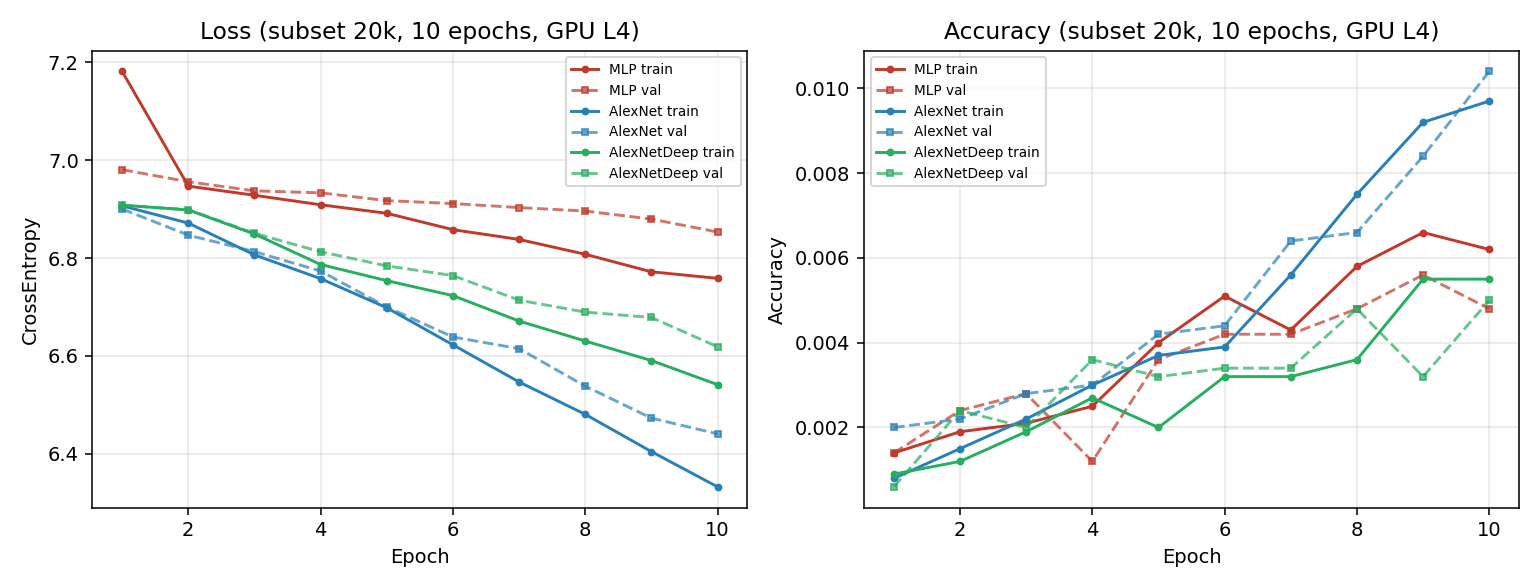
\includegraphics[width=0.95\textwidth]{figures/tb_subset_mlp_vs_alexnet.png}
  \caption{Courbes d'entraînement sur le subset de 20\,000 images pour le MLP,
  AlexNet et AlexNetDeep.}
\end{figure}

\section{ImageNet complet (sbatch)}

Le modèle AlexNet a ensuite été entraîné sur l'ensemble d'ImageNet avec un GPU L4.
Une époque dure environ \textbf{25 minutes}, ce qui représente environ
\textbf{42 heures} pour 100 époques.

\begin{table}[H]
\centering
\small
\caption{AlexNet sur ImageNet complet (job \#9147).}
\begin{tabular}{@{}ccccc@{}}
\toprule
Ép. & Train Loss & Train Acc & Val Loss & Val Acc \\
\midrule
1 & 5,69 & 0,046 & 4,72 & 0,114 \\
2 & 4,73 & 0,121 & 4,13 & 0,186 \\
3 & 4,32 & 0,171 & 3,71 & 0,243 \\
4 & 4,04 & 0,208 & 3,49 & 0,277 \\
5 & 3,84 & 0,235 & 3,30 & 0,308 \\
6 & 3,69 & 0,256 & 3,16 & 0,329 \\
7 & 3,57 & 0,275 & 3,09 & 0,345 \\
8 & 3,47 & 0,289 & 2,98 & 0,365 \\
\bottomrule
\end{tabular}
\end{table}

Les performances progressent vite au début. À l'époque~8, l'accuracy de validation
atteint environ 36,5\,\%, contre 0,1\,\% pour un tirage aléatoire sur 1000 classes.
Le réseau a donc appris des représentations utiles pour classer les images.

Les résultats sur ImageNet complet sont aussi bien meilleurs que sur le subset
de 20\,000 images. Un jeu de données plus grand donne plus d'exemples au modèle
et aide à généraliser. Les augmentations limitent aussi la mémorisation des
exemples d'entraînement.

À l'époque~8, l'écart train/validation reste raisonnable. Rien n'indique encore
un surapprentissage marqué.

\begin{figure}[H]
  \centering
  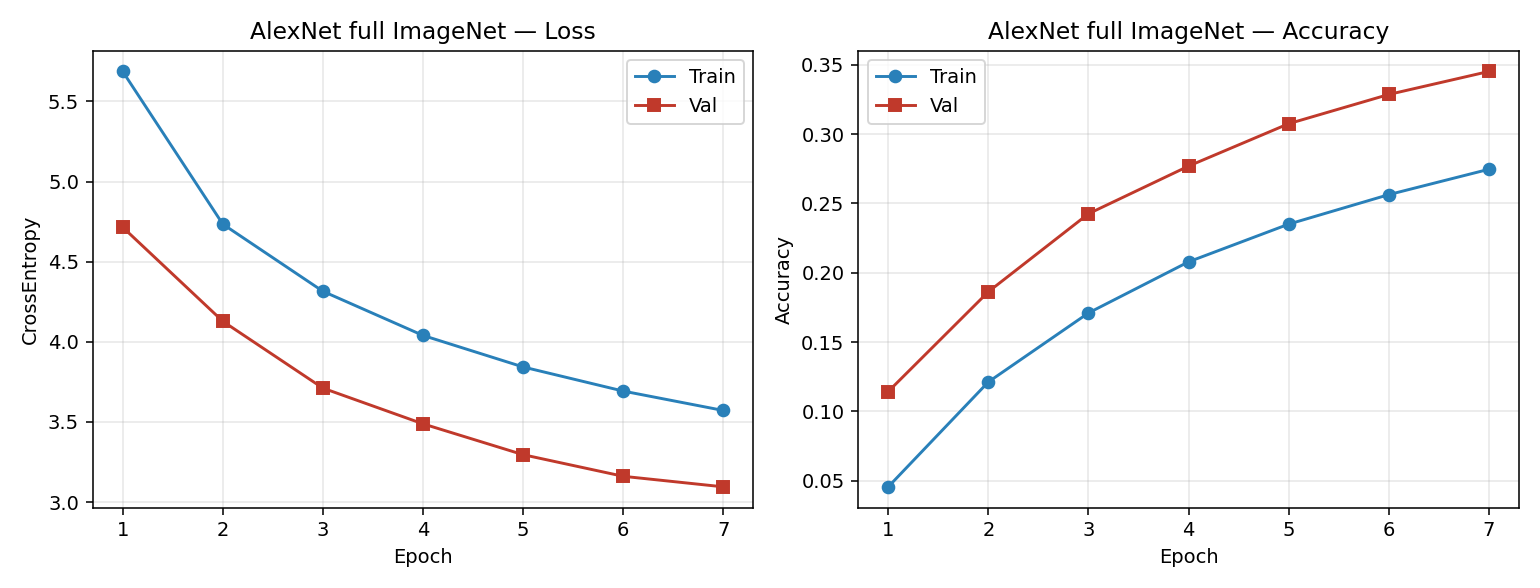
\includegraphics[width=0.88\textwidth]{figures/tb_full_alexnet.png}
  \caption{Courbes d'entraînement d'AlexNet sur ImageNet complet.}
\end{figure}

Au début, la loss de validation peut être un peu plus basse que celle du train.
Ce n'est pas forcément anormal : pendant l'entraînement, le Dropout est actif
et les images sont augmentées, ce qui complique la tâche. En validation, le
Dropout est coupé et le prétraitement est fixe. Le modèle peut donc, un temps,
mieux réussir la validation que le train.

\end{document}
